% Tesis ITAM CLASS -- version 0.1 (13 - Abr - 2015)
% Clase para las tesis del ITAM
% 
% 13 - Abr - 2015 	Victor Martinez 	victor.martinez (at) itam.mx
% LICENSE: Creative Commons SA-BY 3.0
%
%
% Este documento presenta un ejemplo de uso de la plantilla
% El estudiante es libre de modificar este archivo a su gusto
% 
\documentclass{tesisITAM}
\usepackage[utf8]{inputenc}
\usepackage[numbers]{natbib}
\usepackage{array}

\title{ANÁLISIS DE PATRONES DE TRABAJO DE PROGRAMADORES CON DATOS DE INTERACCIÓN}
\author{LUIS CARLOS CRUZ DÍAZ}
\degree{MAESTRO EN CIENCIAS EN COMPUTACIÓN}
\advisor{DR. VÍCTOR MANUEL GONZÁLEZ Y GONZÁLEZ \\* DR. ROMAIN ROBBES}
\year{2016}

\begin{document}

	\pagenumbering{gobble}
	\maketitle
	\publicationrights

	%%%%%%%%%%%%%%%%%%%%%%%%%%%%%%%%%%%%%%%%%%%%%%
	% ABSTRACT
	%%%%%%%%%%%%%%%%%%%%%%%%%%%%%%%%%%%%%%%%%%%%%%

	\begin{abstract}{english}
		Este documento presenta una plantilla para usar en las tesis y tesinas del ITAM. Se provee de manera gratuita y sin ninguna responsabilidad bajo la licencia \emph{creative commons BY-SA 3.0}.
	\end{abstract}

	\begin{abstract}{english}
		In this work we present a template for thesis and titulation works presented at ITAM. It is provided freely and without any responsability under the \emph{creative commons BY-SA 3.0}. 
	\end{abstract}


	\selectlanguage{english}
	\setcounter{page}{1}
	\pagenumbering{roman}

	\tableofcontents
	\listoffigures
	\listoftables
	\newpage

	\pagenumbering{arabic}
	\setcounter{page}{1}

	%%%%%%%%%%%%%%%%%%%%%%%%%%%%%%%%%%%%%%%%%%%%%%
	% CONTENT
	%%%%%%%%%%%%%%%%%%%%%%%%%%%%%%%%%%%%%%%%%%%%%%

	 \chapter{Introducción}
\label{ch:intro}

\begin{chapterquote}{Leslie Lamport}
	Formal mathematics is nature's way of letting you know how sloppy
your mathematics is.
\end{chapterquote}

Este trabajo presenta una plantilla para las tesis y tesinas del Instituto Tecnológico Autónomo de México para los usuarios de \LaTeX. Nace de la necesidad de los matemáticos, actuarios e ingenieros (entre otras carreras) por utilizar un sistema de composición de textos adecuado para su trabajo de titulación. El objetivo es ayudar a la comunidad del ITAM a simplificar el proceso de escritura y edición de sus tesis, tesinas o casos. A continuación describimos a mayor detalle cada una de las partes de la plantilla.

\subsection{Descripción de los archivos}
\begin{enumerate}
\item El archivo \textbf{tesisITAM.cls} define una nueva clase de documento con el mismo nombre. Esta clase se basa en el tipo reporte, el cual se emplea comúnmente para reportes de trabajo, pequeños libros y tesis.

\item El archivo \textbf{macros.sty} define macros y operadores adicionales, como por ejemplo, el argumento mínimo $\argmin$. Además provee un espacio para que el estudiante agregue sus definiciones propias.

\item Este archivo \textbf{introduction.tex} describe el funcionamiento de la plantilla y de los archivos. 

\item El archivo principal \textbf{main.tex} es un ejemplo básico de un archivo de tesis para generar este ejemplo.

\item El archivo \textbf{portada.tex} contiene el código necesario para generar la portada. El archivo \textbf{derechos.tex} contiene el texto para cede de derechos de publicación hacia el ITAM.
\end{enumerate}

\subsection{Características de la plantilla}
La plantilla se basa en el documento tipo reporte. Todas las opciones de la clase \emph{report} pueden ser utilizadas sin ninguna modificación (a4paper, 10pt, etc...). El espaciado del texto se establece a 1.33. Se eliminó la identación del párrafo, y el espaciado entre párrafos fue disminuido. Las sub-secciones se numeran utilizando números romanos. Se define un encabezado para cada página (salvo las que inician un capítulo) donde aparece el número del capítulo y el nombre de la sección.

\subsubsection{Paquetes importados}
La plantilla utiliza los siguientes paquetes: \emph{graphicx}, \emph{amsopn}, \emph{fancyhdr}, y \emph{babel}. El paquete de manejo de idiomas babel es importado con los idiomas \textbf{english} y \emph{spanish} por defacto. Además, se seleccionan las opciones de uso de punto decimal y de nombrar las tablas como tablas y no como cuadros. 

\subsubsection{Opciones de clase}
Se declara una opción adicional de nombre \textbf{tesina} para cambiar la portada a que se declare el trabajo como tesina. 

\subsubsection{Campos para el autor}
Para el autor, se define los siguientes campos: \textbf{title},\textbf{author},\textbf{degree},\textbf{advisor}, y \textbf{year}. \emph{Title} define el título del trabajo de titulación, este título se presenta en la portada y al ceder los derechos de publicación. \emph{Author} define el nombre completo del autor de la tesis. \emph{Degree} se utiliza para establecer la carrera de la cual se va a titular, y debe incluir el texto completo (\emph{i.e.}, Licenciatura en X o Ingeniero en C). \emph{Advisor} recibe el nombre completo (con grado académico) del asesor, tal como se presentará en la portada. \emph{Year} recibe el año de titulación para presentarlo en la portada.

\subsubsection{Generando la portada}
El comando \textbf{\textbackslash maketitle} produce la portada con los campos previamente definidos. Utiliza el logo del ITAM, el cual se debe encontrar en el \textbf{PATH} de \LaTeX (\emph{e.g.}, en el fólder de Figures). 

\subsubsection{Cediendo derechos de publicación}
El comando \textbf{\textbackslash publicationrights} imprime una página con el texto oficial de cede de derechos. Los nombres de la tesis (tesina) y del autor se obtienen de los campos previamente definidos.

\subsubsection{Añadiendo el resumen}
Comúnmente, el resumen (o \emph{abstract}) se debe escribir tanto en español como en inglés. Para esto, se define el ambiente \textbf{abstract} que recibe como parámetro un idioma. En el caso de que el idioma no sea ni inglés ni español, se recomienda que el idioma haya sido previamente importado como opción del paquete babel. En otro caso, el paquete imprimirá una advertencia. 

\subsubsection{Citando a los grandes}
La plantilla define un nuevo ambiente para las citas al principio del capítulo \textbf{chapterquote} que recibe dos parámetros: el autor y el texto. Para un ejemplo, referirse al principio de este capítulo.


\section{Licencia}
Esta plantilla se distribuye bajo la licencia \emph{creative commons BY-SA 3.0}. Esta licencia permite la modificación de cualquier aspecto de la plantilla siempre y cuando se respeten las siguientes condiciones:
\begin{enumerate}
	\item Que se mantenga la atribución del trabajo original, es decir, que se mencionen los autores originales y su afiliación, tal como se hace en el archivo original.
	\item Que todas las modificaciones se hagan públicas y libres de acceso, sin recibir ningún tipo de retribución por el uso o distribución de la plantilla.
\end{enumerate}

\section{Autores}


	 \chapter{Related work}
Now we present a comprehensive analysis of related literature about three main topics: developers' activities, work fragmentation and mining software repositories. All these topics belong to software engineering research and they close each other; some of the cited literature are a convergence of multiple subjects. We start by describing research about developers' activities.

\section{Developers' activities}
In recent years there has been a lot of effort in understanding the way developers work and the challenges they face. With that information we can design tools \cite{CD10, P14, CLQ15, KM06} that offer better conditions on everyday activities. 

Singel et al. \cite{SLV10} surveyed developers to get information of common work practices. They found that programmers spend about half of the time writing code and attending to meetings, and a third or less of the time doing research, configuring, fixing bugs, designing and testing. When shadowing software engineers they were able to get several categories for the activities performed: call trace, consult, compile, configuration, debug, documentation, edit, management, in-house tools, notes, search, source, hardware and UNIX. From these activities, search, looking at the source and editing are the most common in the group of programmers involved in the study. Similarly, LaToza et al. \cite{LVD06} defined a category of activities related to code and motivation: designing, writing, understanding, editing, unit testing, communicating, overhead, other code and non code. The difference between both classifications is that the latter considers collaboration activities with other developers.

Murphy et al. \cite{MKF06} analyzed usage data of multiple programmers with the Eclipse IDE. They found that some of the most commonly executed commands are delete, save, next word and paste. Also, they found that programmers use 11 kinds of refactoring commands (e.g. rename, move, extract and pull up); these commands are often executed via key bindings and exploring the menus.

Program understanding (referred also as program comprehension) involves all kinds of activities meant to better understand the code in development, such as reading the code and documentation, follow a problem-solution-test pattern, interacting with the UI (User Interface), debugging the application, taking notes and more techniques according to Roehm et al. \cite{RTK12}. According to Rugaber \cite{R95}, the difficulty of program comprehension lies in its objective of bridging different concepts, including application domain and solution, the program and the abstraction of design descriptions, and the hierarchical world of programs and the associational nature of human cognition. It is an activity that covers a considerable working time of a developer. There are many studies with estimations of the magnitude of this activity; Fjeldstad and Hamlen \cite{FH83} estimate that about half of the time of software maintaining tasks are spent in program comprehension; Beller et al. \cite{BGZ15} observed that programmers spent 70\% reading code rather than writing, agreeing with Baracchi \cite{B14} on this proportion; Minelli et al. \cite{MMLK14} analyzed usage data and concluded that program comprehension can account from 54\% to 90\% of a working session.

Baracchi \cite{B14} analyzed four kinds of programmer's activities: understanding, editing, inspection and navigation. His findings indicate that the edition activities can be only 20\% of a working session and understanding more than 70\%. Moreover, he classified the working sessions in four groups: Enhancement, Bug-fixing, Refactoring and General. Enhancement sessions are the most common and are followed by the General purpose type of sessions. He uses interaction data with the IDE (Integrated Development Environment).

About testing tasks, Beller et al. \cite{BGZ15} developed a tool to extract usage data from the IDE in order to study the testing practices of software developers. They found that on average they spent 9\% the time testing code, but it can get well below that percentage. Also, developers execute about 5 tests per day roughly every 50 minutes.


On refactoring activities, Murphy-Hill et al. \cite{MPB12} used the Eclipse Usage Data Collector dataset to understand how programmers are using refactoring tools analyzing the patterns of refactoring practices, finding that most programmers do not make deep use of these tools, leaving untouched most of the configuration parameters and performing manually most of the refactoring.

\section{Work Fragmentation}
Work Fragmentation is defined as a break of the work in progress and it is a pervasive phenomenon in all sorts of workers, such as information workers, a group in which developers belong. The activities of an information worker are characterized by spending short time in one task and switching to others frequently \cite{MGH05}. A fragmented working time is constantly interrupted and the frequency depends on the nature of the business \cite{T99}. Some examples of interruptions are emails \cite{BJE05}, notifications \cite{CCH01}, coworkers \cite{LVD06}, meetings \cite{LR05} and oneself \cite{MGH05}.

Mark et al. \cite{MGH05} indicate that interruptions are a common affection of information workers (e.g. administrators, developers and financial analysts). In a field study in an information technology company they found that around 57\% of the working spheres (a day of work is composed of multiple working spheres) are interrupted, and these spheres last only 11 minutes (in average) before going to another sphere or giving place to an interruption. Also, they identified external interruptions (e.g. environment events) and internal interruptions (e.g. taking a break or looking for the solution to a problem). In programmers and analysts the internal and external interruptions occur at the same proportion.

Similar to the previously cited work, much of the research done about interruptions is trough observational studies, experiments and surveys to a broad range of workers. Eyrolle and Cellier \cite{EC00} implemented a laboratory study with telecommunications operators and found that the processing time of a task increases in the presence of interruptions as well as the rate of errors within the first 30 seconds after starting a second task. Bailey et al. \cite{BKC01} also observed a delay on the time spent on a task (subtracting the time spent in interruptions) after having interruptions, and overall a negative effect whose gravity depends on the mental load. They also indicate that interruptions induce annoyance and increase the anxiety and the perceived task difficulty. Burmistrov and Leonova \cite{BL96} executed an exploratory experimental study to measure the impact of interruptions and their complexity on task performance, agreeing with the previous authors that the presence of interruptions increases the time spent on task but also the complexity of the interruption has a significant impact. Cades et al. \cite{CDT07} did an experiment about the complexity or difficulty of interruptions and concluded that more difficult interruptions will lead to greater disruptions, hence increasing the time spent recovering.

Altmann and Trafton \cite{AT04} also found a negative effect of interruptions during an experiment with students performing complex tasks; they attribute the negative effect to the need of recovery called resumption lag, a time invested in the recovery from an interruption. They conclude that having cues available during the resumption lag helps to decrease the time invested in this phase. Iqbal and Horvitz \cite{IH07} mention that resuming a task after an interruption can take from a few seconds to several minutes, depending on the kind of the interruption (e.g. messaging and emails); they observed that in average the user takes around 5 minutes to respond to an alert, from 9 to 8 minutes are spent in the interruption and 16 minutes recovering from it. They also present an interruption life cycle involving 4 phases: 
\begin{itemize}
	\item Preparation: time between an alert and the suspension of the task.
	\item Diversion: time spent in the interruption.
	\item Resumption: end of the interruption and resumption of the interrupted task.
	\item Pre-interruption: time spent on the activity before the arrival of a new alert.
\end{itemize}
Parnin \cite{PD10} applied a survey to software developers to better understand the impact of interruptions. According to the results, the most common technique to recover after an interruption is reading the code and navigate backwards in the code until recovering the previous work. For some programmers this is not enough they and use tools to find recent changes in the code. Most of them leave notes, physical or electronic, about the progress before the interruption. Moreover, starting to code after the interruption takes between 10 to 15 minutes, a similar observation to the results of Sanchez et al. \cite{SRV15} who performed an analysis of the interruptions and the impact of productivity with interaction data.


\section{Mining Software Repositories}
The core of this work is within the Mining Software Repositories research area, which can be defined as the extraction of information from different artifacts (e.g. source code, control version logs, documentation and bug reports) that are produced throughout the software development cycle \cite{H04}. This term is not alien to data mining, so the intentions are extracting knowledge and discovering patterns in the data using a set of techniques and algorithms for this goal \cite{FPG96}.

The software repositories can be found in different formats \cite{H08}:
\begin{itemize}
	\item \textbf{Historical repositories}, with information obtained throughout the evolution of a project, e.g., bug reports, emails and control version logs.
	\item \textbf{Runtime repositories}, like deployment information, performance reports and application usage data.
	\item \textbf{Code repositories}, which is access to the source code from a version control such as SVN and Git, or online platforms such as SourceForge or Github.
\end{itemize}

Although some of this repositories are used to keep control of changes and procedures, they are rarely used to make decisions. One of the goals of the Mining Software Repositories field is allowing static repositories to be a guide for decision making, for it is possible to discover important information and patterns that can help predict the future performance of the team and the quality of the product in development \cite{H08, ZZW05}. Each stage of the development of software releases data that can be exploited to make timely decisions. Recently, Hassan \cite{HX10} appointed the name of \emph{Software Intelligence} for all the practices involving Mining Software Repositories within companies.

\subsection{Predicting errors}
There are tasks that have a greater impact with these practices. For example, the project administration can make decisions based on facts and tendencies reflected in the data that can be visualized with metrics, or even predict future events like modules prone to errors based on recent activity.

Related to the latter, there is a great effort in using this data for quality assurance. Khomf et al. \cite{KDZ12} analyzed product release data of the Firefox navigator while the developers were migrating from a traditional release scheme to an agile methodology and found that, though there are the same amount of errors, the users tend to identify them early and the failures are fixed quicker.

Error prediction is another example of the interest in quality. The work made by Nagappan et al. \cite{NBZ06} and Finaly et al. \cite{FPC14} are similar approaches for error prediction using complexity metrics, which are measures of the source code (e.g. the number of lines, functions and classes). Both works agree about the difficulty of predicting errors using solely these metrics and in the low precision of the proposed models. Zimmerman and Nagappan \cite{ZN08} obtained better results considering the structure of the system and the relation between classes, creating a network and obtaining metrics from the related graph. The graph was built identifying the code dependencies of the program, where the nodes are classes and the edges the dependencies between them. From the graph they obtained metrics like the number of nodes, the amount of dependencies in relation to a node and the distance to a node. They found that, although the complexity metrics have better correlation with the amount of errors, the graph metrics can predict well with regression models.

Meneely et al. \cite{MWS08} also used networks to predict errors in modules based on product release data, but instead of representing classes as nodes, they represent the programmers that worked on the project and the edges are created when two of them work in the same piece of code. The authors also used graph metrics to train a predictive model, obtaining a precision of 81\%.

\section{Usage data }
Another example of data that can be captured is the usage data (also called interaction data) between the programmer and the development tools \cite{SnipesETALASD}, which is log of the execution of events within the IDE (Integrated Development Environment). The IDE provides tools to execute tasks effectively, such as navigation between classes and methods, continuous compilation, refactoring, automated testing and debugging, all designed to assist the programmers' productivity. The Figure \ref{fig:ide} shows a screenshot of the Eclipse IDE

\begin{figure}[!ht]
	\centering
	
	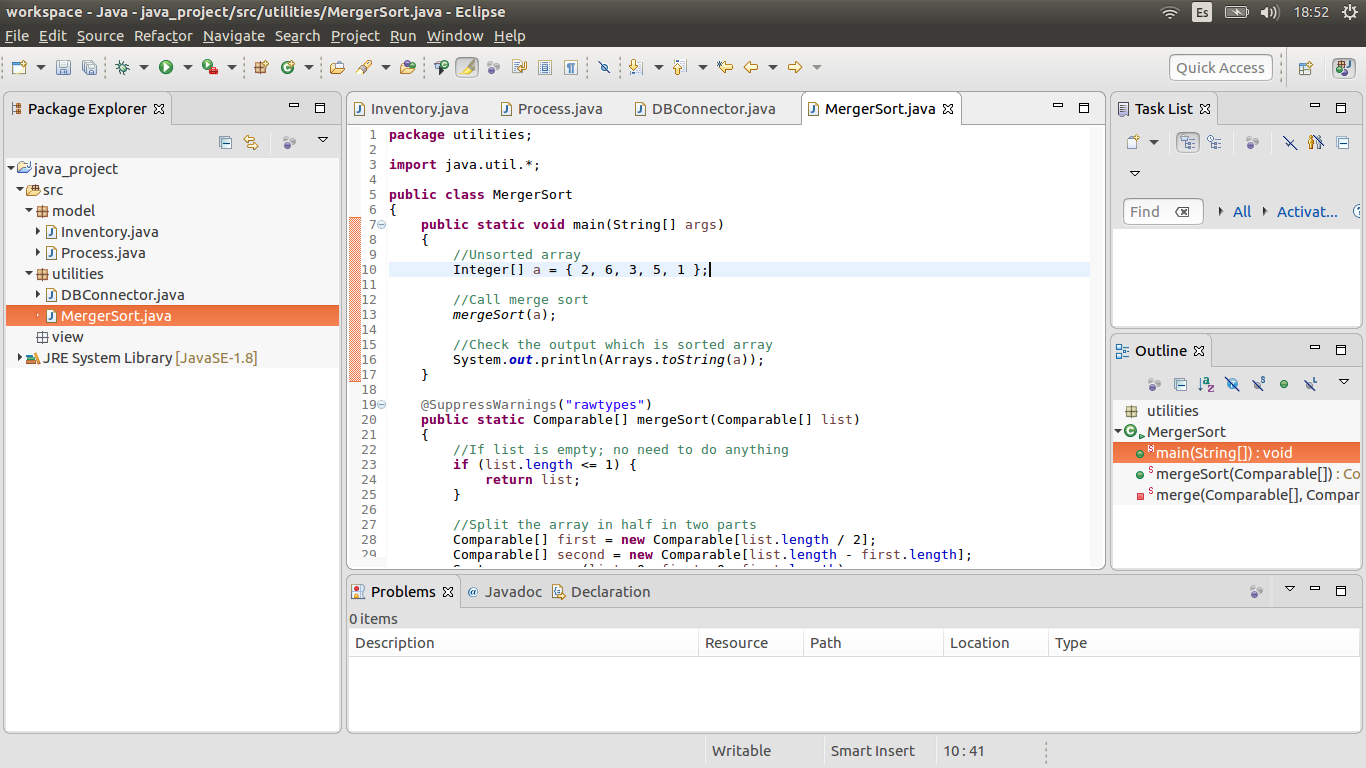
\includegraphics[width=\linewidth,clip=, angle=0]{Figures/IDE}  
	
	\caption{User interface of the Eclipse IDE. }
	\label{fig:ide}
\end{figure}

The usage data is composed of the interactions between the programmer and the IDE, and can include the description of executed commands (e.g. copy, paste, delete and save); the opening or closing of files; clicks, change of line and navigation around text; usage of tools, and more. Generally, everything is stored in a log with date, time and an identifier for the user. As a complement it can contain the name of the class and/or the function where it was executed and the type of the event. The Table \ref{tbl:example_usage_data} shows an fragment of the Eclipse Usage Data Collector dataset with four attributes to represent the user, what kind of command was executed, the description of the command and the date and time of execution.

\begin{changedforreviewerlong}
\begin{table}[ht!]
	\small
	\caption{Example of usage data from the Eclipse Usage Data Collector. }
	\label{tbl:example_usage_data}
	\centering
	\begin{tabular}{p{0.8cm}|p{1.7cm}|p{6.3cm} | p{3cm}} 
		\hline 
		\emph{User} & \emph{Kind} & \emph{Description} & \emph{Datetime}\\  
		\hline 
		\hline 
		5017 & command & org.eclipse.ui.edit.text.goto.lineEnd & 2008-12-15 16:20:28\\
		\hline
		5017 & editor & org.eclipse.wst.jsdt.ui.CompilationUnitEditor & 2008-12-15 16:20:30 \\
		\hline
		5017 & command & org.eclipse.ui.edit.copy & 2008-12-15 16:20:36 \\
		\hline
		5017 & command & org.eclipse.ui.edit.paste & 2008-12-15 16:20:45 \\
		\hline
		5017 & command & org.eclipse.ui.edit.text.goto.lineEnd & 2008-12-15 16:20:46 \\
		\hline
		
	\end{tabular}
\end{table}
\end{changedforreviewerlong}

It is possible to command the IDE to capture usage data to have better understanding, to a low level, of the activities of the programmer \cite{SnipesETALASD}. Eclipse and Visual Studio are examples of IDEs that provide an API (Application Programming Interface) that allows to register all the commands and actions that are begin executed. It is not necessary to build an application to capture the data, for there are several options to collect it like Eclipse Usage Data Collector \cite{MPB12}, Mylyn Monitor \cite{KM06} and Codealike \cite{CLQ15}. It is possible to start a study with existing data from previous projects. An example is the available information in the Eclipse archives about the Usage Data Collector, a dataset of more than 1 million users and 2,000 million registered events.

%\subsection{Productivity metrics}
%Given that the available information about usage data can tell the history of activity of the programmer, one of the most used metrics is the total active time, without the time consumed in interruptions, like the study by Sanchez et al. \cite{SRV15}. The active time is also considered by the focus function of Codealike, which increases when more activity is registered. The focus level is a metric used by this tool to measure the productivity and tries to model the concentration of the user. Prolonged time without registered activity o time outside the IDE are identified as interruptions, being the number of interruptions another metric.

%When it is possible to classify the events by its type it can be used metrics like the editions per minute or selections per minute. It is also common to use debugging per minute as metric, like the research by Carter and Dewan \cite{CD10}. Moreover, Sanchez et al. \cite{SRV15} identified that during sessions without interruptions the proportion of edition events is superior than navigation events, so one of their conclusions is that it is a good indicator of productivity. This tell us that a productive programmer spends more time coding and less time exploring the code.

%Codealike \cite{CLQ15} also uses a classification of events to quantify the technical debt when a class or function has more navigation events and debugging than edition events, which indicates that the element can be a bottle neck for the project. 

\subsection{Research with usage data}
Kersten and Murphy \cite{KM06} proposed a tool that keep the context of the task being performed by the programmer and make it visible to help in the navigation around elements. The context is a graph of classes, modules and functions that are relevant for the current task and that are needed to complete it. Each element related to the task has a weighted value that is created with a model of the degree of interest of that element according to the task. The degree of interest which is the amount of recent activity that the programmer made on an element; increases with the frequency of interactions on an element and decreases when the interactions stop. Later, it is shown to the programmer a list of elements ordered by the value. In a field study with programmers, the authors obtained qualitative and quantitative results that indicate an increase of productivity when having context of the task in progress, specially in big systems with many programmers collaborating.

Fritz et al. \cite{FMH07} did a research about the possibility of inferring whether the programmer has knowledge of the code or not by quantifying the degree of knowledge, as extension to the work done by Kersten and Murphy \cite{KM06}. In a field study, they monitored the activity of 19 programmers and applied a weekly survey for three weeks. They concluded that when the programmer has knowledge of code (according to the surveys) there is a high degree of interest, concluding that the usage data can be used to identify this phenomenon.

Carter and Dewan \cite{CD10} inquire about the possibility of identifying a programmer stuck or having problems, which is when there is no progress despite of the effort, under the hypothesis that the activity of the programmer will give out evidence of this state. During an experiment with students in a programming course, the participants were asked to indicate when they were facing problems during programming tasks and while usage data was being captured. From the data they obtained metrics of the number of edition, navigation and debugging events per minute, and with the data labeled where the programmer was stuck, they trained several machine learning algorithms. The best result was obtained with a decision tree, which correctly predicted the "in problems" state the 92\% of the times, concluding that it is possible to identify this state with usage data.

Minelli et al. \cite{MMLK14} performed an analysis about the process of program comprehension and compared the results with the literature. Based on interaction data, they labeled the segments of the working sessions of programmers according to the activity, specifically in sectors where the programmer was navigating around classes, editing code, inspecting objects and reading the code. Then, they split the sessions in segments and quantified them according to the activity performed and concluded that the program comprehension activity was underestimated by previous research, for the results indicated that this activity covers (in average) 65\% to 90\% of the working sessions, against a previous estimation of 35\%.

%Sanchez et al. \cite{SRV15} used interaction data to perform an empirical analysis of the impact of work fragmentation on productivity, identifying lapses of time without recorded activity as interruptions and quantifying the productivity according to the number of edition and selection events, and the proportion of edition events against selections. They found that productivity decreases as the number of interruptions increases in a working session, and that in sessions with prolonged interruptions the productivity tends to be lesser in comparison with sessions with only short or none interruption. In session without interruptions the productivity is triplicated, but they are only the 2\% of all the sessions of a programmer.

\begin{changedforreviewerlong}
In the previous sections we made a review of the literature about three main topics: 2ork interruptions, developers' activities and usage data. We started by introducing related work to developer's activities and then made a transition to work fragmentation and work interruptions, which are topics closely related, one affecting the other. After that we introduced the Mining Software Repositories research area that analyzes software engineering phenomena with data extracted throughout the software development life cycle. An example of it is usage data that describes the interactions with the developmental tools. We use this data to offer answers to the questions regarding interruptions and developers' activities.

This work is an intersection of the three, and offers answers to some questions about the first two topics by analyzing usage data. 
\end{changedforreviewerlong}

	 \chapter{Data and Methodology}
The results presented in this work are based on the information that can be extracted from usage data. We used two datasets to provide answers to our research questions that come from different sources but are similar in the kind information contained. In this Chapter we describe the data and methodology used for knowledge extraction. 
\begin{changedforreviewerlong}
We used the \emph{Knowledge Discovery in Databases} process \cite{FPG96}, a set of iterative steps composed of Selection, Preprocessing, Transformation, Data Mining and Interpretation. This chapter will cover the Selection, Preprocessing and Transformation steps. In the latter Chapters we will give details about the Data Mining and Interpretation steps.
\end{changedforreviewerlong} First, we describe the data in the following section, which also covers the Selection step of the methodology.

\section{Description of the data}
It is important to first describe the data in terms of the attributes, magnitude and context of extraction. In the following subsection we describe in detail the characteristics of the datasets, limitations and some inferences we can obtain.

\subsection{Eclipse Usage Data Collector}
The Usage Data Collector (UDC) dataset is a large compendium of information about interaction data from users of Eclipse, collected from December 2008 to August 2010, with the intention to keep track of how programmers are using the IDE. The framework listens to the events triggered by the user or the system, such as: edition and navigation commands; the startup of a plug in; or the closing of the platform. To be more specific, UDC collects information about loaded bundles, commands accessed via keyboard shortcuts, actions invoked via menu or tool-bars, perspective changes, view usage and editor usage. The UDC is a large dataset that contains information of around 1,800,000 users, and has a total of 2,323,233,101 unique rows with 5 attributes each. Table \ref{tbl:att_udc} shows a description of the attributes.

This dataset only contains information of the execution of commands within the IDE and we do not have more context about the programmers or environments. Judging by the registry of events, there is a mix of programmers of different nature such as Java SE, Java EE and Web developers. There are also programmers that use other kind of languages such as PHP, SQL and Ruby. We assume that this data corresponds to programmers of all levels of expertise, from students to professionals.


\begin{table}[ht!]
	\small
	\caption{Attributes of the UDC dataset. }
	\label{tbl:att_udc}
	\centering
	\begin{tabular}{p{2.5cm}|p{7cm}} 
		\hline 
		\emph{Attribute} & \emph{Description} \\  
		\hline 
		\hline 
		UserId &  Unique number that identifies a user \\
		\hline
		What & The action of the event (deactivated, activated, opened, executed, etc.)  \\
		\hline
		Kind & What kind of event was executed (workbench, view, command, etc.)  \\
		\hline
		BundleId & Description of the event's package  \\
		\hline
		BundleVersion & Version of the bundle's event  \\
		\hline
		Description & Description of the event\\
		\hline
		Datetime & Date and time in UNIX format\\
		\hline
	\end{tabular}
	
\end{table}

We used the pre-processed version of the data that is published on Google BigQuery, by Murphy-Hill et al. \cite{SnipesETALASD}. This is an alternative version of the original UDC dataset, which is cleaned and preprocessed, so that the cleaning phase is simpler and focused on our needs. 

Due to the magnitude of the dataset we only worked on a fragment of it. We took a subset of the data from 1,000 random users. We delimited the query to obtain only those events dispatched by the user, ignoring system events. We also ignored the BundleId and BundleVersion, leaving only the attributes UserId, What, Kind, Description and Datetime. From this query we extracted 4,321,349 unique events, which are around $0.18\%$ of the whole dataset.

\subsection{Codealike and ABB}
Codealike \cite{CLQ15} is a tool that monitors the activity of the user and later offers analytics and insight about the programmer's productivity and working patterns. This tool is installed in the IDE (Eclipse and Visual Studio) and listens to the events executed by the user and system, similar to UDC. It captures almost the same kind of events (e.g. edition, navigation and tool usage). Shortly after the capture of events, the user can observe information derived from his activity through a website.

Corvalius (the Argentinian company that created Codealike) is collaborating with ABB, a multinational corporation operating mainly in robotics, power and automation technology areas. The ABB's Software Engineering Research Group is using Codealike to obtain information from its developers with the objective of improving productivity and software quality. We had access to a dataset corresponding to the monitoring of 87 programmers between May and October of 2015 comprising 15,597,697 unique events. The main dataset that contains the registry of executed commands has the attributes described in the Table \ref{tbl:att_abb}.

The data was extracted from Visual Studio via Codealike and the events correspond to .NET programming languages, such as C\# or Visual Basic. Similar to UDC, it only contains a registry of executed commands and no information about the developers, except for the country of origin judging by the email domain that was provided. The programmers were invited to use Codealike at will, so the amount of data collected varies among users. We assume that this data corresponds to professional programmers working for the same company and under similar circumstances. The latter meaning that they are more likely to have same or similar equipment, methodology, tools and working hours. However, we can not be certain about any of these assumptions.

\begin{table}[ht!]
	\small
	\caption{Attributes of the ABB dataset. }
	\label{tbl:att_abb}
	\centering
	\begin{tabular}{p{2.5cm}|p{7cm}} 
		\hline 
		\emph{Attribute} & \emph{Description} \\  
		\hline 
		\hline 
		Username &  Unique identifier of the user \\
		\hline
		Timestamp & Date and time of the execution  \\
		\hline
		Event & Identifier of the event's description  \\
		\hline
		Category & Unique identifier of the event's category \\
		\hline
	\end{tabular}
	
\end{table}

The actual description of the events is stored on a different file, so we use the values of the Category and Events attributes to extract it. In this case, all the attributes are needed. From hereafter this dataset will be referred to as ABB.

\section{Methodology}

The following subsections will give detail about the Preprocessing and Transformation steps.

\subsection{Preprocessing}
During the Preprocessing stage we performed mainly two tasks: data cleaning and classification. The cleaning tasks are trivial, for the data is in good conditions. However classifying the events is a complicated task that requires careful inspection and multiple iterations. The tasks involving data cleaning diverge between datasets, so we give details about this step separately. But the classification of events follows the same process for both datasets and is described afterwards.

\begin{changedforreviewerlong}
\subsubsection{UDC}
First, we added a field with the duration of every event (time elapsing between one event and the next one). This task is required to identify the interruptions and working sessions later, and it is related to the first four research questions. Then, we sorted the data by UserId and Datetime. This was required because, by default, the user's data is mixed and we need it not only chronologically correct but also sorted by users to tag the working sessions of every user without interferences. We also filled the description for the events that indicate the activation or deactivation of the Eclipse's workbench, which were the only ones with that issue.

\subsubsection{ABB}
The Preprocessing for ABB is also simple. As with UDC, we added a duration in seconds to every event. Then, we extracted the Description from a second dataset, according to the Event and Category, and created a new attribute. We changed the Description to lowercase and removed curly braces and other special characters. Finally, we removed events executed by the system and ordered the data by Username and Datetime. It is necessary to have a clear description to add the classification, which is described in the next subsection.



\subsection{Classification of events}
The classification of events adds a class or type to each of the events recorded in the data. It is a crucial task with the following motivations:
\begin{enumerate}
	\item Having more than a thousand different events, it reduces the complexity of managing each of the events separately. At the end, although they execute different tasks, they have a goal in common that we try to capture when assigning a classification.
	\item Some of the metrics used throughout this study rely on the existence of a classification that describes the general behavior of the developer.
\end{enumerate}

To classify the events, we look into the description to see what it can tell us about the event. We worked with two kinds of classifications:
\begin{itemize}
	\item A general classification to identify between Edition and Selection events. It is used to describe the behavior of the programmer in a general manner. It is used in the analysis of interruptions of work.
	\item A detailed classification to tag the nature of every event. It is used when we need a detailed inspection of the activities. We use it in both analyses (interruptions of work and developers' activities).
\end{itemize}

The two classifications will help us provide better answers to our research questions, for some of them require doing analyses in detail and others can be seen from a general perspective. The general classification is derived from the detailed classification, and it is easily performed by setting as Selection all the events except those that perform text edition, text navigation and refactoring tasks; this set of events describe the kind of activities performed when editing code, while the rest involve navigation around classes, the opening of views and selection of graphical elements. To identify those events we rely on the detailed classification described in the Table \ref{tbl:detailed_events}.

\end{changedforreviewerlong}

\begin{table}[ht!]
	\small
	\caption{Description of the detailed classification of events. }
	\label{tbl:detailed_events}
	\centering
	\begin{tabular}{p{2cm}|p{4.5cm}|p{4.5cm}} 
		\hline 
		\emph{Classification} & \emph{Description} & \emph{Examples} \\  
		\hline 
		\hline 
		Edit-Text &  Text edition events & Copy, Paste and Delete. \\
		\hline
		Text-Nav & Events executed when navigating around text. & LineUp, LineDown and LineEnd.  \\
		\hline
		High-Nav & Navigation of high level  (around classes and views). & GoToDefinition, NextTab and GoToSuperclass \\
		\hline
		Debug & Events executed during debugging sessions. & StepInto and StepOver. \\
		\hline
		Search & Events executed when searching for objects and text. & Search, Find and FindReplace. \\
		\hline
		Refactoring & Events executed when restructuring code. & Encapsulate, Rename and MoveField. \\
		\hline
		Testing & When testing (e.g. unit tests) is executed through a framework. & ExecuteTest and TestResults. \\
		\hline
		Control & Execution of version control tasks. & Compare, ViewChanges and CommitChanges. \\
		\hline
		Clean-Build & Tasks performed by the IDE to build and execute a solution.  & Build and Run. \\
		\hline
		File & Events executed during the management of files. & Open, Close and SaveChanges. \\
		\hline
		Tools & Execution of specialized tools and plugins. & DatabaseDesigner, Codealike and UIDesigner.\\
		\hline
	\end{tabular}
	
\end{table}

To assign a detailed classification we use the description. In both datasets the description has the format \emph{path.to.class.ListenerClass}. It contains the path to the class that works as listener of the event and executes the required task. The packages and class name give out information about the nature of the event.

%With that in mind, we created a set of rules that adds a classification to every event according to the name of the class and/or the name of the path. For example, in UDC we label as Text-Nav all the events that have \emph{ui.edit.scroll} in the description, and in ABB we label as High-Nav all the events whose class name is \emph{NextTab}. Sometimes it was required to create special rules for certain events but most of the time we were able to set rules for several of them. This was an iterative process that required careful inspection of the results.


\subsection{Transformation }

\begin{changedforreviewerlong}
The objectives of the transformation phase are identifying the working sessions and calculating a set of metrics and time series for each; we use time series because they allow us to model the temporal nature of working sessions and we use several of them to represent the different sources of information. Then every session is decomposed into chunks or segments of smaller time than sessions; this allows us to see detailed patterns when analyzing developers' activities in RQ5 and RQ6.


First, we identified interruptions using the duration or time interval of every event. It is required by the research questions regarding the interruptions of work analysis. This is an important task and it is convenient to define the two kinds of interruptions we use in this work:
\end{changedforreviewerlong}

\begin{itemize}
	\item \textit{Interruption.} We define empirically an interruption as a pause of activity of duration $\geq 3$ minutes. This is based on previous work where we observed that short interruptions lasted usually this long \cite{GM04}. Shorter values would risk classifying periods of inactivity (such as a programmer reading source code) as interruptions.
	
	\item \textit{Prolonged interruption.} Based on additional observations from this work, we defined a prolonged interruption as one lasting for more than 12 minutes. These thresholds are also supported by the Activity Theory models of Kaptelinin and Nardi \cite{KaptelininN07}. This study presented work fragmentation at two different levels: actions and activities. Interruptions originated after a period of around three minutes of sustained attention to the previous action were considered when people were switching at the level of interactions with artifacts of people. Interruptions originated after a period of twelve minutes of sustained attention to a previous activity were considered when people were switching at the level of interactions with projects or topics. They are only used in RQ2.
\end{itemize}

To identify working sessions we look for interruptions as well, but only those that last for more than 4 hours. Any segment of activity surrounded by interruptions with that duration is labeled as a session. However, in order for the segment to be valid it must be of at least 30 minutes of duration. This is a task that concerns all the research questions.

Then, for every session we created several time series representing the execution of events by detailed classification. Taking the minute as time unit, we counted the number of events executed on every minute and created eleven time series, where the amplitude is the number of events. The interruptions were treated differently; they are also contained in a time series of its own but the amplitude is the duration of the interruption and every observation represents the minute of occurrence. 

After that, the next step is to calculate a number of metrics for every session that measure the activity of the programmer. These metrics will later be used to get answers to RQ1, RQ2 and RQ3. They can be seen from two perspectives, first the metrics for the characterization of interruptions:
\begin{itemize}
	\item \textit{Number of interruptions}:  counts all the interruptions that occur in a development session.
	\item \textit{Duration of interruption}:  it is the time duration in minutes of the each interruption. 
\end{itemize}

And the metrics that describe the productivity and activity:
\begin{itemize}
	\item \textit{Productive work time:} the duration of a development session, subtracting the duration of all the interruptions present in the session, to control for inactivity.
	\item \textit{Number of edits per minute:} the total number of edits events, divided by the productive work time to control for length of the session. This is an indicator of user activity during the session.
	\item \textit{Number of selections per minute:} it is the total number of selection events, divided by the productive work time. Also an indicator of activity.
	\item \textit{Edit ratio:} the number of edits divided by the sum of edits and selections, as used by Kersten and Murphy \cite{KM06}; an efficient developer spends less time exploring code and more time editing it.
	%\item \textit{Proportion of events:} it is the count of events by detailed type divided by the total of events executed in the session. There are a total of 11 values for this metric, but it is only used in RQ5 and RQ6.
\end{itemize} 

\subsection{Transformations Regarding Developers' Activities}
The transformation tasks described previously are performed (mostly) to both datasets and are needed to answer all of the research questions. Here we describe one final step of the process that only applies to RQ5 and RQ6, about developers' activities.
\begin{changedforreviewerlong}

The last task of the transformation phase is to split the sessions into smaller activity frames to do analyses of the programmer's activity in detail for RQ5 and RQ6. In order to do that, we split the time series of every session into time segments of 3 to 5 minutes of activity that we will call chunks. We selected this time frame so that activities that are rare or require a small amount of events do not get obscured by common activities. Moreover, it was observed that some tasks can be performed within 3 minutes before moving to another one \cite{GM04}.

It was necessary to recreate the time series for the chunks, and then calculate the proportion of events by detailed type; there are a total of 11 detailed types, so every chunk had 11 extra metrics representing the proportion of each detailed type. After this, every user has a set of sessions (with their respective time series) and every session has a set of chunks.
\end{changedforreviewerlong}

\subsection{Characterization of Working Sessions}
We can observe some statistics about the resulting sessions in the Table \ref{tbl:stats_sessions}. UDC contains much more sessions, but in average they are shorter (4.11 hrs) than the sessions in ABB (7.33 hrs). However, in both cases the actual time spent working in the IDE is much less, being in average of 64.29 minutes for UDC and 166.08 minutes in ABB. The average number of interruptions per session is larger in ABB (25.40) than in UDC (9.52), which is in relation to the size of the sessions, but in ABB the interruptions tend to be shorter (10.74 minutes).

\begin{table}[ht!]
	\small
	\caption{Statistics of sessions in UDC and ABB. }
	\label{tbl:stats_sessions}
	\centering
	\begin{tabular}{p{3.5cm}|p{2cm}|p{2cm}} 
		\hline
		\emph{Statistic} & \emph{UDC} & \emph{ABB} \\
		\hline
		\hline
		Number of sessions & 6,405 & 1,182 \\
		\hline
		Number of observations & 2,848,270 & 2,449,227 \\
		\hline
		Number of users & 621 & 69 \\
		\hline
		Number of chunks & 43,769 & 23,624 \\
		\hline
		Avg. duration & 4.11 hrs. & 7.33 hrs. \\
		\hline
		Avg. productive time & 64.29 min & 166.08 min \\
		\hline
		Avg. of interruptions & 9.52 & 25.40 \\
		\hline
		Avg. duration of inte. & 18.94 min & 10.74 min \\
		\hline
	\end{tabular}
\end{table}

After the Selection, Preprocessing and Transformation we end up with a set of sessions, each with its corresponding time series and metrics. The metrics will be used mostly in the research questions about work interruptions and the time series are useful for the two topics. Also, the sessions were decomposed into chunks or smaller frames of time, which will allow us to investigate in detail the activities of programmers. Having the data ready, we can proceed to analyze and answer our research questions.


	 \chapter{Results}
\label{ch:intro}

\section{Activities and working patterns}
For the first part of this section we present a characterization of working sessions at different levels, extracting the information from the ABB and UDC datasets. The ABB data corresponds to full-time developers, so we assume that they follow certain working patterns and have common activities. For that, we expect to see an homogeneous behavior among the developers.

In contrast, UDC dataset contains more variety and different profiles of programmers, so it might be troublesome to find specific patterns.

\subsection{Characterizing working sessions}
We defined a working session as a lapse of recorded activity surrounded by interruptions of large duration (8 hours), to model a day of work. However, in many cases the extracted sessions contained an interruption of moderate length in the middle, so we set a threshold of 4 hours to split this kind of sessions. At the end, we had 1,585 sessions with an average duration of 4.7 hours ($s=3.58$).

From the transformation phase, every session is composed of time series and other attributes. There is a time series to represent the interruptions, where the amplitude is the duration of every interruption, and 11 more series whose amplitude is the amount of events of every type per minute. Every data point of the time series is equal to a minute of activity in the data, meaning that all the time series have the same length. In average this length is of $121.61$ minutes ($s=147.81$). This is also refereed as productive time, or the total time that the programmer spent working on the IDE without being interrupted.

A lot of the time of a working session is wasted in interruptions, or time segments of at least 3 minutes without recorded activity. In average every session has 18 interruptions (sd=21.17) with an average duration of 10.78 minutes. As for the total time consumed in interruptions, the average is of 190 minutes (sd=137.19), which is more than half the average duration of a session.

\subsection{Using focus data}
Complementary to the dataset, we had access to the focus data of a smaller group of programmers from ABB. This dataset contains the focus level (a value between 0 and 1) per minute that Codealike uses in its tool as an inference of the concentration of the user. The focus is calculated according to two functions: one to increase the value when the programmer makes use of the IDE, and a second one as a decay function, that is applied when the programmer is inactive. Therefore, when the user is active the value decreases and the contrary when he is not using the IDE.

This can be used as a summarization of the activity the user and to get very general information. For example, the Figure \ref{fig:prod_hours} shows the total focus per hour from all the programmers. We can see that the 14 hours seems to be the more productive time, for is the hour with the higher value of focus or the time with more usage of the IDE. There is a decrease at the 16 hrs., and increases a again to later abruptly drop at 21 hrs. The activity is lower between the 21 and 8 hours.

\begin{figure}[!ht]
	\centering
	\begin{tabular}{c}
		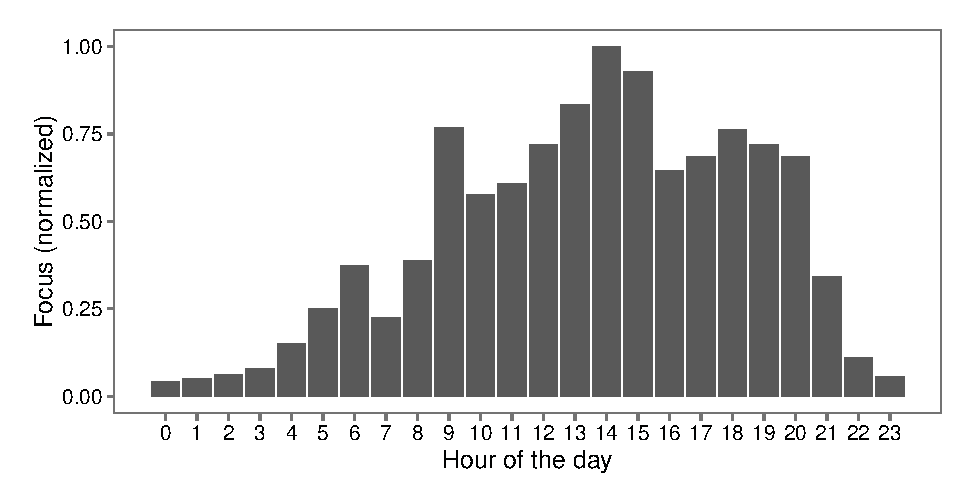
\includegraphics[width=1\linewidth,clip=, angle=0]{Figures/productive_hours_focus} 
	\end{tabular}
	\caption{Histogram of productivity per hour according to the focus data.}
	\label{fig:prod_hours}
\end{figure}

With this information we can also see the evolution of productivity throughout the days of the week. The Figure \ref{fig:prod_days} shows the sum of focus level (normalized) for every day of the week. There is not a great difference aside from the weekend, but there is a slight decrease the days Monday and Friday, and the most productive days are Tuesday and Thursday.

\begin{figure}[!ht]
	\centering
	\begin{tabular}{c}
		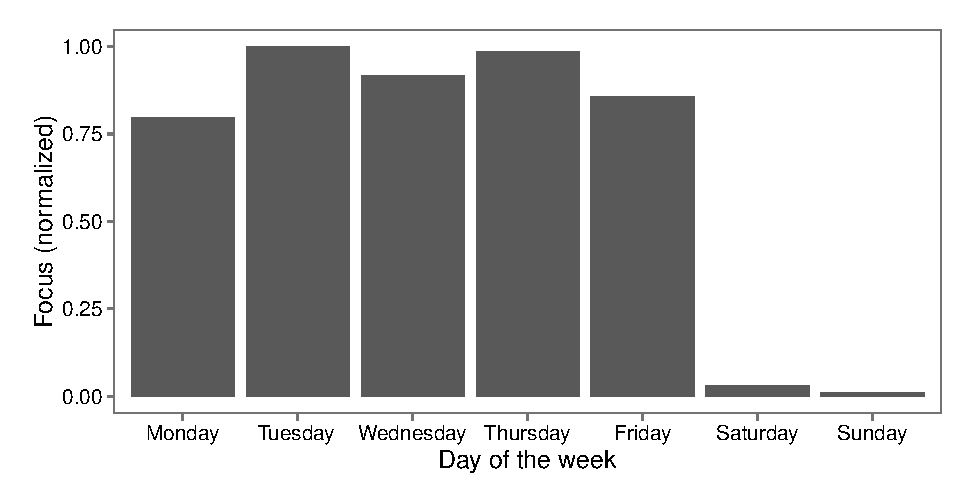
\includegraphics[width=1\linewidth,clip=, angle=0]{Figures/productive_days_focus} 
	\end{tabular}
	\caption{Histogram of productivity per day according to the focus data.}
	\label{fig:prod_days}
\end{figure}

%\subsection{Decomposed working sessions}
%To explore the working patterns at a finer level, we decomposed the sessions to small chunks of 3 to 5 minutes of activity without interruptions. This resulted in 31,973 different observations, each with their respective time series and proportion of events by type. 

%\subsection{Characterizing developers}
%We have information from 69 programmers, each offering an average of 22 working sessions. We do not have more information about them, like roles and working hours

\subsection{Identifying types of activities}
In order to identify the types of activities the programmers perform, we split every working session into smaller activity time frames of 3 to 5 minutes of length. For each of this new chunks of the sessions we recreated the time series and calculated the proportion of events per type, which is the count of events of type $t$ divided by the total count of events in that chunk. After this, we obtained a total of 31,727 chunks.

The nature (or the type) of a chunk is defined by the amount of events of certain type in comparison with others. For example, for the activity of programming we expect a high proportion of events of edition, and probably also navigation around text and classes. The challenge is to know what threshold set to differentiate between two types of activities that might use the same kind of events, i.e. reading and programming could both use text navigation events. Also, if we try to define a set of activities according to experience and related work, we might be ignoring certain characteristic activities of this group of programmers or forcing one to exist. For this reasons we decided to implement clustering algorithms with the chunks, taking the proportion of events as the attributes. So, every observation contained 11 different attributes whose values are between 0 and 1.

As we didn't know how many types of activities there were, we discarded the algorithms that require the number of clusters as parameter, like K-means and K-medians. From the rest of algorithms, we chose Mean shift because: (1) in contrast with Affinity propagation (our other option) the time complexity is lower, and (2) the Mean shift technique performs one last step to unify very similar clusters. The importance of the second point will be discussed later.

An issue with Mean shift is that the size of the observations has a big impact in the results: a small population can offer more variety of clusters, and a big population could be clustered around one or two centers. Mean shifts creates the clusters by estimating a density function over a region of size given by the bandwidth, a parameter of the algorithm. So, the bandwidth also has an effect on the results.

It is difficult to know which are the appropriate parameters and sample size because, for we do not know what are the results. To tackle this, we took the following approach:
\begin{enumerate}
	\item From the observations, select a random sample size $n$.
	\item Execute the Mean shift technique with the random sample.
	\item Store the resulting clusters.
	\item Repeat $k$ times steps 1 to 3.
	\item Filter the clusters to eliminate very close centers according to the Euclidean distance and a threshold $d$. 
	\item Discard clusters that only appeared in one execution.
\end{enumerate}

The fifth step is done by measuring the distance of a cluster with the rest and selecting the group of clusters with a distance lesser or equal to $d$. Then, we calculated the median of the attributes of all the clusters in that group and substituted the group with the new cluster created from the medians. 

With this approach we were able to observe very common clusters corresponding to frequent activities like programming and debugging, and also activities that only occur on special occasions or that are not very common within a working session.


With $n=300$ and $k=150$, the Table \ref{tbl:activities} shows the resulting clusters. We selected the corresponding activity by inspecting the closeness of the center to the attributes: the higher the value, the most events of that type. For example the Debugging activity has a value of 0.90 (from a range between 0 to 1) for the debug type; the rest of the activities have a value $<0.20$ for that type of event. Next, we describe each of the activities discovered via clustering:

\begin{itemize}
	\item \emph{Debugging}. The most common activity has a big value for the debug type (0.90). It is composed of events meant to execute and control debugging sessions.
	\item \emph{Programming}. It has the greatest values for the edit and text-nav types (0.62 and 0.24, respectively). It contains text edition and text navigation events and it's the second most common activity.
	\item \emph{Navigation}. This activity has a high value for the high-nav type (0.85). It is often related to comprehension tasks.
	\item \emph{Version-control}. It has a high value for the control type (0.89).
	\item \emph{File-management}. It has a high value for the file type (0.86).
	\item \emph{Tool-usage}. This activity represents the execution and usage of tools within the IDE with different objectives i.e. the management of databases, user interface design and architecture diagrams design. It has a high value for the tools type (0.91)
	\item \emph{Search}. It has the higher value for the search type (0.91) and to a lesser extent for edition and text-nav (0.10 and 0.11 respectively).
	\item \emph{Refactoring}. It has a high value for the refactoring type (0.90) and to a lesser extent for edition, text-nav and high-nav (0.13, 0.15 and 0.13 respectively)
	\item \emph{Testing}. It has a high value for the testing type (0.95) and to a lesser extent control and file types (0.35 and 0.19 respectively).
\end{itemize}

\begin{table}
	\caption{Activities found via clustering.}
	\label{tbl:activities}
	\centering
	\begin{tabular}{c c c c}
		\hline 
		\emph{Activity} & \emph{Amount of chunks} & \emph{Users} & \emph{Times found}\\  
		\hline 
		\hline 
		Debugging & 40.62 \% & 59 & 150\\
		\hline
		Programming & 35.53 \% & 58 & 150 \\
		\hline
		Navigation & 18.67 \% & 61 & 140\\
		\hline
		Version-control & 1.85 \% & 33 & 150\\
		\hline
		File-management & 1.60 \% & 45 & 2 \\
		\hline
		Tool-usage & 0.59 \% & 28 & 149\\
		\hline
		Search & 0.49 \% & 32 & 14\\
		\hline
		Refactoring & 0.34 \% & 13 & 17\\
		\hline
		Testing & 0.30 \% & 17 & 58\\
		\hline
	\end{tabular}
\end{table}

Once we had every chunk of a session labeled with the corresponding activity, we did an analysis of the evolution of the activities throughout a working session. For that, we split every session into 10 phases and counted the activities by type on each of the phases from all the sessions. The Figure \ref{fig:activities_phases} shows a line plot with the evolution of four selected activities (Programming, Debugging, Version-control and Testing) throughout the 10 phases of the sessions.

\begin{figure}[!ht]
	\centering
	\begin{tabular}{c}
		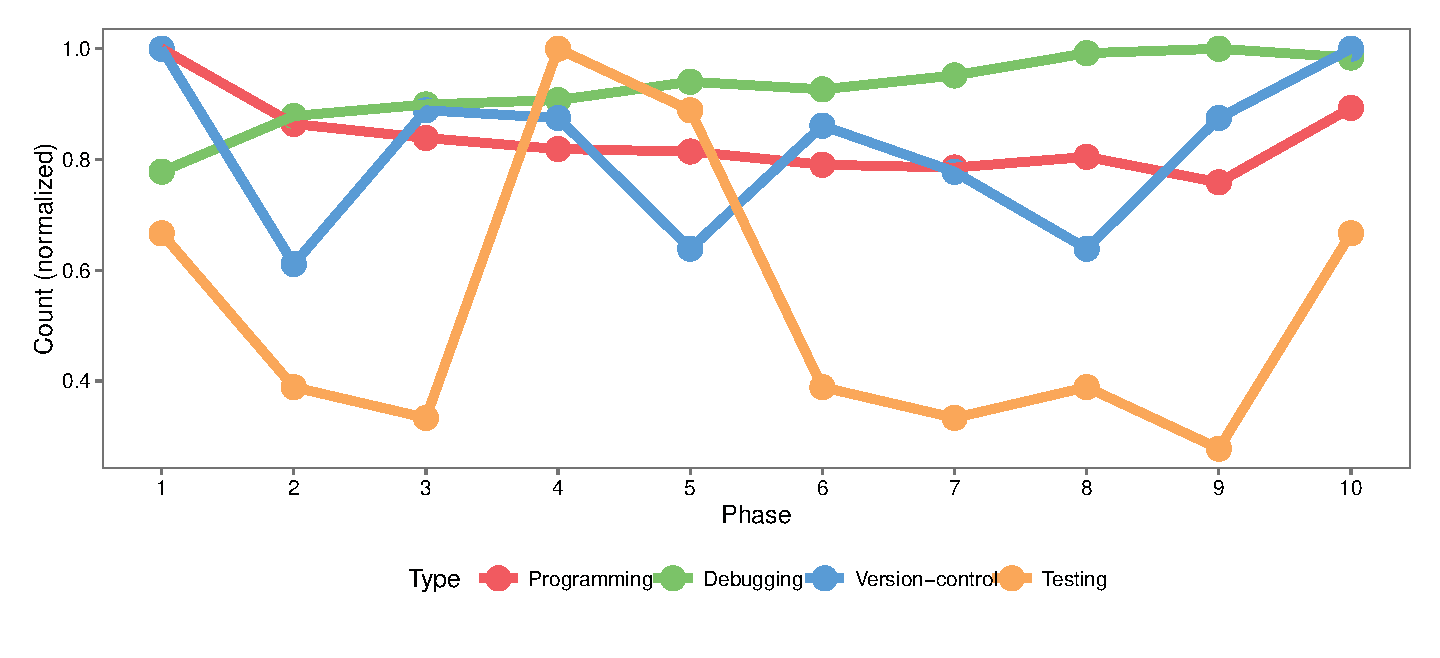
\includegraphics[width=1\linewidth,clip=, angle=0]{Figures/activities_phases} 
	\end{tabular}
	\caption{Evolution of the activities throughout the sessions.}
	\label{fig:activities_phases}
\end{figure}

We can observe that Programming starts high and gradually decreases towards the end of the session, and the contrary occurs with Debugging, whose highest point is at the 9th phase. There is a negative correlation between these two activities ($r=-0.76$), possibly meaning that as the programmer advances with the task the programming necessities are reduced but increases the need for debugging and checking the correctness of the program. In contrast, the Navigation activity (not shown in the plot) has a positive correlation with programming ($r=0.74$).

The Version-control activity seems to have an irregular behavior, being high at the beginning and ending of the session. The reason could be that at the beginning the programmer obtains the latest version of the program, while at the end he commits the final version after the working session. In the middle there are some peaks that might be different checkpoints that the programmer reaches as he has progress in the task. 

As for the Testing activities, there s an obvious peak at the middle of the session and lower activity in the rest.


	% \chapter{Conclusions}

In this work we analyzed the impact of interruptions on the productivity and working patterns of developers as seen in usage data. This data came from two sources: the Usage Data Collector of Eclipse, with information of a variety of programmers, and a second dataset from Codealike that contains information of professional software developers from ABB.

Overall, we conclude that it is possible to observe in usage data the effects of events that occur in a working place (in our case interruptions) and the activities performed by developers. The results we obtained can be matched to observations from observational studies and experiments, so that we gained confidence in using this kind of information to understand complex phenomena. With that in mind, it may be possible in the near future to have better programming tools that learn from the activities of the user and offer assistance in common challenges and problems that developers face in a daily basis, and be able to mutate according to the circumstances. The results on work fragmentation covered in this thesis is under submission to the Journal of Software: Evolution and Process.

As future work, we consider valuable applying the same procedures while obtaining feedback from the developers. By doing so we can assure that our conclusions based on usage data are validated by the input from the developers. Also, we would be able to obtain more variables and enrich our results.

In Chapter 1 we defined a set of research questions as objectives grouped in two approaches: effect of interruptions and working patterns. Now we present a summary of our conclusions for each of the research questions. 

\textbf{RQ1: What is the relationship between the observed interruptions and the observed developer productivity?} 

We observed an inverse relationship between the number of interruptions and the productivity metrics. The editions per minute metric shows a stronger effect, specially in the first three groups involving from 0 to 3 interruptions. Beyond that point the effect seems smaller but still decreasing towards the groups with a high number of interruptions. This can be seen in the selections per minute as well and to a lesser extent in the edit ratio. We conclude that the number of interruptions has a negative effect on the productivity of developers, reducing the amount of activities performed.

\textbf{RQ2: Is the observed relationship more pronounced in the presence of prolonged interruptions?}

Then we investigated whether the length of the interruption has an increased effect, specifically if prolonged interruptions ($\geq$ 12 minutes) has a greater impact than shorter interruptions. Considering that the number of the interruptions has an effect, we created seven groups consisting of sessions with 1 to 7 interruptions and each was split into two additional groups according to the proportion of prolonged interruptions: low proportion and high proportion. We observed that the metrics show higher values when having a low number of interruptions and a low proportion of prolonged interruptions. So, we conclude that prolonged interruptions have a more disruptive effect than short interruptions.

\textbf{RQ3: What is the observed relationship in the vicinity of interruptions?}

Next, we look into the vicinity of interruptions and the behavior of the metrics 30 minutes before and after the interruption occurs. We observed an abrupt decrease of productivity in the immediate minutes around the interruption, approximately 10 minutes around it. Based on the literature, we are seeing the effect of the preparations before the interruption, and afterwards all the activities involved in the recovery of the context of the task. Moreover, we found three patterns of interruptions: positive, negative and neutral. This is an indication that not every interruption is disruptive, for some of them might be used to find solutions and answers.

\textbf{RQ4: What events are more common during recovery time?}

The last question involving interruptions is a follow up of the observations in the past research question. We observed a change of the metrics after the interruption, a phase called resumption or recovery time in the literature. Also we saw different patterns when having positive and negative interruptions. We delved deeper into the recovery time and analyzed which are the most common activities in this phase after a positive and negative interruption. We found that after a positive interruption there are more assertive actions like text edition and refactoring; we hypothesize that this is when the developer has the solution to a problem he faced before the interruption. On the other hand, after a negative interruption the actions are more related to program comprehension, like navigation around classes and debugging the program; we hypothesize that this occurs when the interruption has a disruptive effect the developer must perform the necessary activities to recover from it. We backed our findings with observations from the literature.

\textbf{RQ5: What kind of activities can be identified with interaction data?}
Having performed an analysis of work interruptions, we changed the subject to activities and working patterns and used the two available datasets. The first question in this context was meant to discover what kind of activities we can find in the data according to executed events. Using small time frames of activity, we executed clustering techniques to find them. In the UDC data we found eight activities and in the ABB data only six. Five activities appear in both datasets (Debugging, Programming, Navigation, Versioning and Tool usage) and the rest are unique. The percentages also differ between datasets and it can be due to the different tools used to capture them and the kind of programmers of the samples. Most of this activities have been characterized in observational studies and we lack information to detect activities related to collaboration between developers and interactions outside of the IDE.

\textbf{RQ6: What working patterns during a session are commonly performed by developers?}

Once we had all the activities performed by the developers, we split every working session into three phases and cluster them to find patterns of activities. We found several centroids (patterns) but the most common correspond to working sessions were the programmer mostly performs programming activities, program comprehension or general activities (multitasking). These three kind of activities can be observed in both datasets. This patterns of activities can be related to types of working sessions observed in observational studies.





	%%%%%%%%%%%%%%%%%%%%%%%%%%%%%%%%%%%%%%%%%%%%%%
	% APPENDIX
	%%%%%%%%%%%%%%%%%%%%%%%%%%%%%%%%%%%%%%%%%%%%%%
	\appendix
	% \include{Chapters/appendixA}

	%%%%%%%%%%%%%%%%%%%%%%%%%%%%%%%%%%%%%%%%%%%%%%
	% BIBLIOGRAPHY
	%%%%%%%%%%%%%%%%%%%%%%%%%%%%%%%%%%%%%%%%%%%%%%
	\clearpage
	\addcontentsline{toc}{chapter}{References} %Añadimos la bibliografia a la lista de contenidos.
	
	%%%%%%%%% Referencias usando el sistema embedido %%%%%%%%%%%
	% e.g. (Ejemplo tomado de https://en.wikibooks.org/wiki/LaTeX/Bibliography_Management)
	%
	 \bibliographystyle{chicago}
	 \bibliography{mybib}

\end{document}